\documentclass[pra,twocolumn,preprintnumbers,amsmath,amssymb,nofootinbib,floatfix,longbibliography]{revtex4}

\usepackage{graphicx, bm, tikz, braket, mathrsfs}
\usepackage[breaklinks]{hyperref}

\makeatletter

\def\graphicscale{\twocolumn@sw{0.3}{0.4}}
\def\graphicthreescale{\twocolumn@sw{0.3}{0.4}}
\newcommand{\rev}[1]{\textcolor{red}{#1}}

\begin{document}

\title{Notes}

\author{}
\affiliation{}

%\date{}

\begin{abstract}
\end{abstract}
\maketitle

\section{Model}

We consider the following Kitaev Hamiltonian:

\begin{equation}
	\label{HKitaev}
	\hat H_K =-\mu_i \sum_{x=1}^L \hat c_x^\dagger \hat c_x
    -\sum _{x=1}^{L-1} \Bigr[\hat c_x^\dagger \hat c_{x+1}
	\hat c_x \hat c_{x+1} + {\rm h.c.} \Bigr]  \,\,.
\end{equation}

To monitor the critical behavior close the critical point
$\mu_c = -2$ we introduce the following scaling variables:
\begin{align}
	\label{scalvar}
	\kappa_i & = (\mu_i - \mu_c) L^{y_{\mu}} \,\,, \\
	\eta & = T L^{z} \,\,;
\end{align}
where in the last equation, we introduce the initial
temperature $T$ of the system and $z=1$ is the dynamical
critical exponent. Since we take the Kitaev chain in
equilibrium with the temperature $T$, the initial density
matrix corresponds with the Gibbs mixture:
\begin{align}
	\label{Gibbs}
	\hat \rho_T & = e^{-\beta \hat H_K} \,\,,\\
	\beta & = \frac{1}{T} \,\,.
\end{align}
To evaluate the correlations in the state $\rho_T$, we take
the steady state obtained by the limit $t \to +\infty$ of
the solution associated with the Lindblad equation.
The dissipation term is given by a set of equal thermal
bath homogeneous coupled with each site
\cite{P-2022-otto}.\\

Thus, introducing the two-point correlations functions as:
\begin{align}
  \label{corrs}
  C(x,y) &={\rm Tr}\Bigr[\rho_T\hat c^\dagger_x \hat c_y
						+  {\rm h.c.}\Bigr]\,\,,\\
  P(x,y) &={\rm Tr}\Bigr[\rho_T\hat c_x\hat c_y +
    {\rm h.c.}\Bigr] \,\,;
\end{align}
in the initial thermal steady state, their behavior is
described by the scaling laws:
\begin{align}
	\label{scalTcorr}
	C(x,y;\mu_i,T) &=L^{-2y_c} {\cal C}(x/L, y/L, \kappa_i,
    \eta) \,\,;\\
	P(x,y;\mu_i,T) &=L^{-2y_c} {\cal P}(x/L, y/L, \kappa_i,
                                     \eta) \,\,.
\end{align}



\section{Out-of-equilibrium dynamics}

\subsection{Unitary dynamics}

\begin{figure}[!htb]
  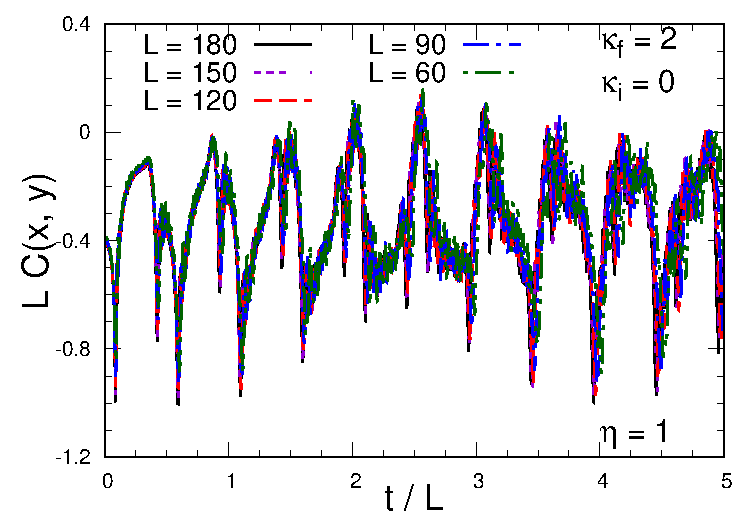
\includegraphics[width=0.95\columnwidth]
  {figs/Cqthk0q2e1.pdf}
    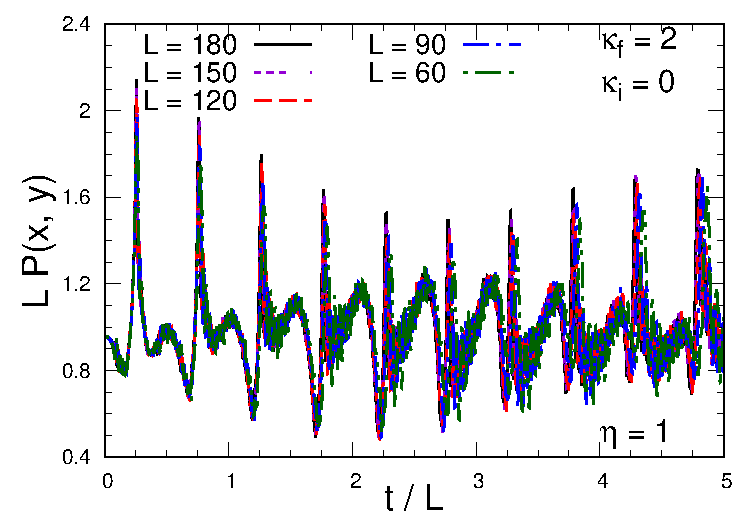
\includegraphics[width=0.95\columnwidth]
    {figs/Pqthk0q2e1.pdf}
    \caption{Scaling behavior of the two-points
    correlations functions $C(x,y,t)$ (top) and $P(x,y,t)$
    (bottom) for $x=L/3$, $y=2L/3$  keeping the scaling
variables $\kappa_i=0$,
    $\kappa_f=2$, $\eta =1$ fixed in function of $tL^{-z}$,
    up to system size $L=180$.}
  \label{qthk0q2e1}
\end{figure}

Starting from the state introduced above, at $t=0$, we
change suddenly the value of the chemical potential $\mu_i$
to a final value $\mu_f$. In other words, we perform a
quench protocol on the Hamiltonian (\ref{HKitaev}) from an
initial value to another one. This process lead to a
reformulation of the Bogoliubov bases in which the time
evolution operator acts. \\
This operator is unitary because the state is not in
contact with any thermal bath. The corresponding scaling
law in Eqs. \ref{scalTcorr} become:
\begin{align}
  \label{scalTquench}
  C(x,y,t;\mu_i,\mu_f,T) & = L^{-2y_c} {\cal C}(x/L,y/L,
  tL^{-z},\kappa_i,\kappa_f, \eta) \,\,,\\
  P(x,y,t;\mu_i,\mu_f,T) & = L^{-2y_c} {\cal P}(x/L, y/L,
  tL^{-z},\kappa_i,\kappa_f, \eta) \,\,;
\end{align}
where $\kappa_f$ is the scaling variable associated the
final chemical potential $\mu_f$.\\

\subsection{Thermal dissipation case}

Now, in the case in which we turn on a homogeneous thermal
dissipation mechanism, the time evolution is not more
unitary, but it is the interplay between two processes:
\begin{itemize}
  \item the Quench protocol;
  \item the dissipation arising from equal thermal baths
  with temperature $T_b$.
\end{itemize}
To write the scaling laws, we have to define new scaling
variable whose aim is to tune the dissipation with the
critical behavior:
\begin{align}
	\label{TbScalvar}
	\eta_b & = T_b L^{z} \,\,;\\
	\Gamma & = \gamma L^{z} \,\,.
\end{align}
The $\gamma$ factor is simple the dissipation coupling
which enters in the following Lindblad equation:
\begin{align}
   \label{EQLindblad}
   \frac{\partial}{\partial t} \rho &= -i\,\Bigr[ \hat H,
      \rho \Bigr] + \mathbb{D}[\rho]\,\,,\\
  \mathbb{D}[\rho] = \gamma \sum_k & (1-f(\omega_k))
  \,\biggr[ 2\hat b_{k} \rho \hat b_{k}^\dagger - \Bigl\{
  \rho, \, \hat b_{k}^\dagger \hat b_{k} \Bigl\} \biggr]+
  \notag \\
  + \,\,\gamma \sum _k &
  f(\omega_k)\,\biggr[ 2\hat b_{k}^\dagger \rho \hat b_{k}-
  \Bigl\{ \rho, \, \hat b_{k} \hat b_{k}^\dagger \Bigl\}
  \biggr]
\end{align}
where the Bogoliubov operator $\hat b _k$ corresponds with
the quasi-particle annihilation operator of the
$k^{\rm th}$ mode. Moreover, they are associated with the
Hamiltonian after the quench, i.e. when the chemical
potential is equal to $\mu_f$.


\begin{figure}[!htb]
  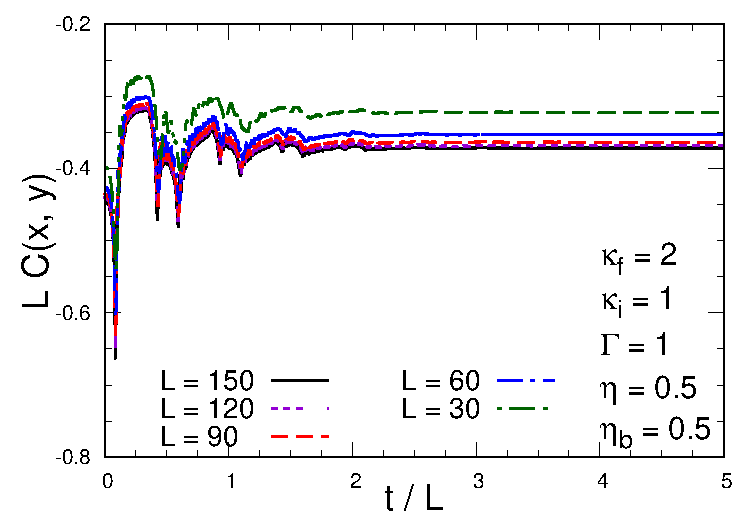
\includegraphics[width=0.95\columnwidth]
    {figs/LCk1q2e050t050S1000.pdf}
  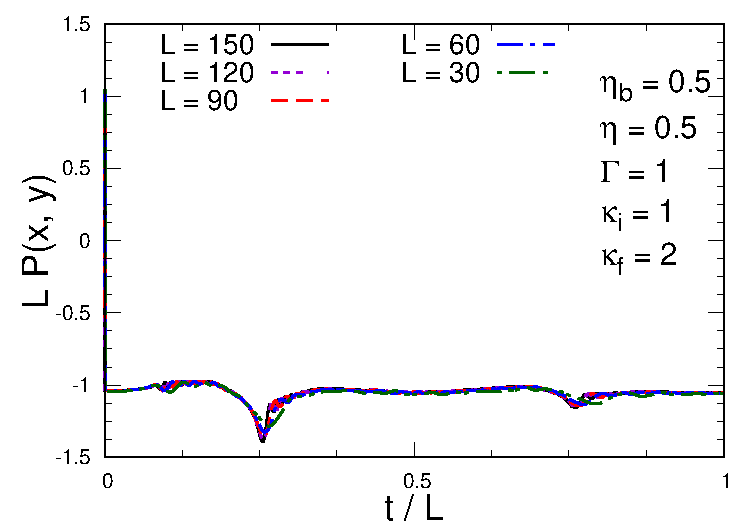
\includegraphics[width=0.95\columnwidth]
    {figs/LPk1q2e050t050S1000.pdf}
  \caption{Scaling behavior of the two-points
    correlations functions $C(x,y,t)$ (top) and $P(x,y,t)$
    (bottom) for $x=L/3$, $y=2L/3$  keeping the scaling
    variables $\kappa_i=1$, $\kappa_f=2$, $\eta =0.5$,
    $\eta_b=0.5$, $\Gamma = 1$ fixed in function of
    $tL^{-z}$, up to system size $L=150$.}
  \label{k1q2e050t050S1000}
\end{figure}

\begin{figure}[!htb]
  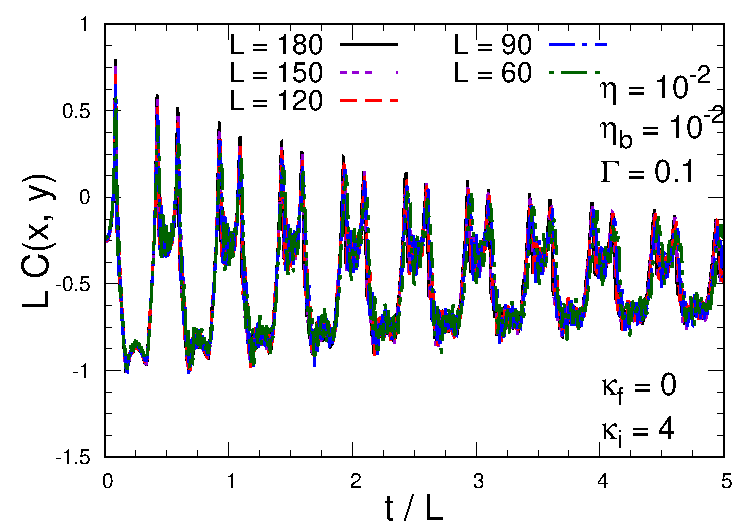
\includegraphics[width=0.95\columnwidth]
    {figs/LCk4q0e001t001S0100.pdf}
  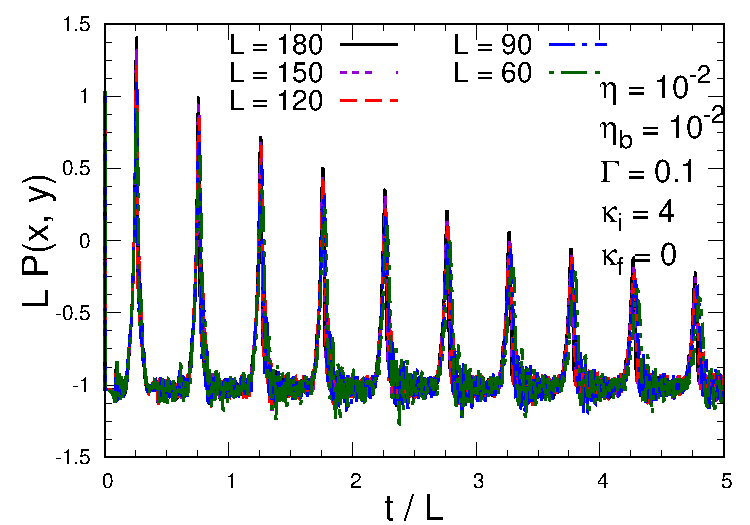
\includegraphics[width=0.95\columnwidth]
    {figs/LPk4q0e001t001S0100.pdf}
  \caption{Scaling behavior of the two-points
    correlations functions $C(x,y,t)$ (top) and $P(x,y,t)$
    (bottom) for $x=L/3$, $y=2L/3$  keeping the scaling
    variables $\kappa_i=4$, $\kappa_f=0$, $\eta =0.01$,
    $\eta_b=0.01$, $\Gamma=0.1$ fixed in function of
    $tL^{-z}$, up to system size $L=180$.}
  \label{k4q0e001t001S0100}
\end{figure}


\begin{figure}[!htb]
  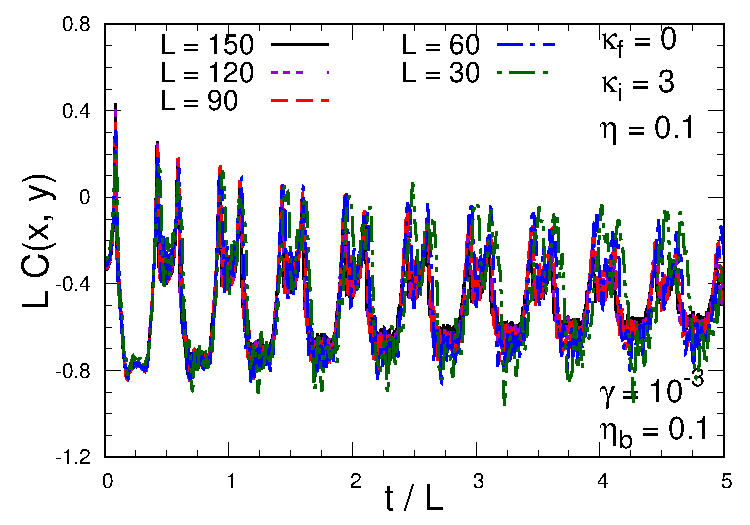
\includegraphics[width=0.95\columnwidth]
    {figs/LCk3q0e010t010g0001.pdf}
  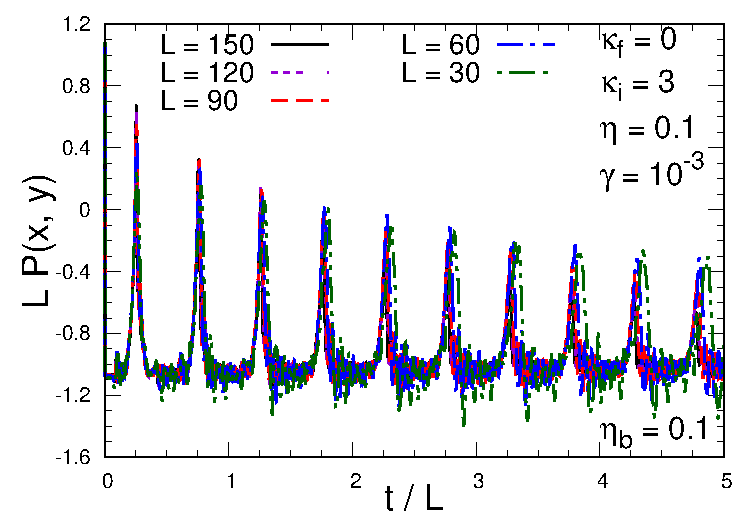
\includegraphics[width=0.95\columnwidth]
    {figs/LPk3q0e010t010g0001.pdf}
  \caption{Scaling behavior of the two-points
    correlations functions $C(x,y,t)$ (top) and $P(x,y,t)$
    (bottom) for $x=L/3$, $y=2L/3$  keeping the scaling
    variables $\kappa_i=3$, $\kappa_f=0$, $\eta=0.1$,
    $\eta_b=0.1$, $\gamma=10^{-3}$ fixed in function of
    $tL^{-z}$, up to system size $L=150$.}
  \label{k3q0e010t010g0001}
\end{figure}

\begin{figure}[!htb]
  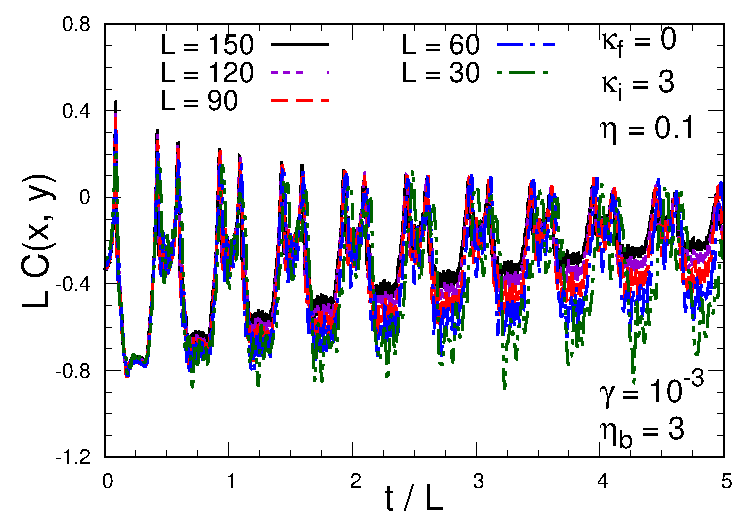
\includegraphics[width=0.95\columnwidth]
    {figs/LCk3q0e010t300g0001.pdf}
  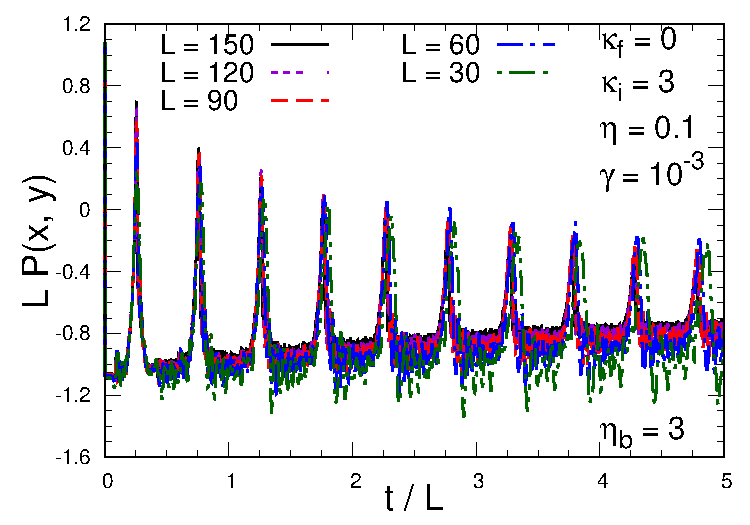
\includegraphics[width=0.95\columnwidth]
    {figs/LPk3q0e010t300g0001.pdf}
  \caption{Scaling behavior of the two-points
    correlations functions $C(x,y,t)$ (top) and $P(x,y,t)$
    (bottom) for $x=L/3$, $y=2L/3$  keeping the scaling
    variables $\kappa_i=3$, $\kappa_f=0$, $\eta=0.1$,
    $\eta_b=3$,$\gamma=10^{-3}$ fixed in function of
    $tL^{-z}$, up to system size $L=150$.}
  \label{k3q0e010t300g0001}
\end{figure}





%%%%%%%%%%%%%%%%%%%%%%%%%%%%%%%%%%%%%%%%%%%%%%%%%%%%%%%%%%%


%\bibliography{refs.bib}

\end{document}






































